\section{Einführung in die Programmierung}

\begin{frame}{Vorstellung}
\begin{itemize}
	\item Name
	\item Studiengang 
	\item Programmiererfahrung allgemein
	\item Programmiererfahrung Python
	\item Erwartungen
\end{itemize}
\end{frame}

\begin{frame}{Organisatorisches}
    \begin{itemize}
        \item Anwesenheitspflicht
        \item Teilnahmebestätigung (Zertifikat)
        \item "Regeln"
        \item Codio
        \item Skript
    \end{itemize}
\end{frame}

\begin{frame}{Ablauf}
\begin{tabular}{ l l }
	14.00 - 14.30 & Erwartungen und Vorkenntnisse\\
	14.30 - 15.00 & Einführung in Python und Einrichtung der Umgebung \\
	15.00 - 15.30 & Variablen und Operatoren\\
	15.30 - 15.45 & Pause \\
	15.45 - 16.45 & Schleifen \\
	17.00 - 18.00 & Bedingungen\\
	
\end{tabular}
\end{frame}

\begin{frame}{Ablauf}

\begin{tabular}{ l l }
	10.15 - 10.30 & Besprechung Tagesplan\\
	10.30 - 11.00 & Wiederholung \\
	11.00 - 11.15 & Typconventionen\\
	11.00 - 11.30 & Listen \\
	11.30 - 11.45 & Pause\\
	11.45 - 12.00 & Funktionen\\
	12.00 - 13.00 & Anwendung alles bisher Gelernten\\
	13.00 - 14.00 & Mittagspause\\
	14.00 - 15.30 & Datein einlesen/ausgeben\\
	15.30 - 16.00 & allgemeine Theorie\\
	
\end{tabular}
\end{frame}

\begin{frame}{Die Programmiersprache Python}
\begin{columns}
    \column{0.5\textwidth}
    \begin{itemize}
        \item Warum Python?
            \begin{itemize}
                \item flache Lernkurve, sehenswerte Ergebnisse bereits nach dem ersten Tag
                \item verankert in Forschung und Wirtschaft
                \item der englischen Sprache sehr änhlich
            \end{itemize}
    \end{itemize}
    \column{0.5\textwidth}
    \centering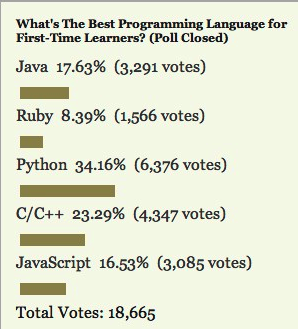
\includegraphics[scale=0.5]{images/best_lang} 
    \hyperlink{https://lifehacker.com/five-best-programming-languages-for-first-time-learners-1494256243}{\tiny{Quelle: lifehacker.com}}
\end{columns}
\end{frame}

\defverbatim{\pythonenglish}{%
\begin{lstlisting}[frame=none,basicstyle=\fontsize{9}{11}\ttfamily]
languages = ["C", "C++", "Java", "Python", "Fortran"]
modern_languages = \ 
    list((x for x in languages if x is not "Fortran"))
\end{lstlisting}
}
\begin{frame}[standout]
    \pythonenglish
\end{frame}

